\chapter{Järjestäminen}

Järjestäminen on keskeinen algoritmiikan ongelma,
jolle on käyttöä sekä itsenäisenä algoritmina että
laajemman algoritmin osana.
Voimme ratkaista monia ongelmia järjestämällä
ensin aineiston, minkä jälkeen voimme hyö\-dyntää
järjestystä tavalla tai toisella.

Yksinkertaiset algoritmit järjestämiseen toimivat
ajassa $O(n^2)$, ja ne perustuvat kahteen sisäkkäiseen
silmukkaan.
Voimme kuitenkin järjestää taulukon myös tehokkaammin
ajassa $O(n \log n)$, mikä mahdollistaa järjestämisen
käyttämisen tehokkaiden algoritmien suunnittelussa.

Tässä luvussa tutustumme ensin järjestämisen teoriaan
ja erilaisiin järjes\-tämisalgoritmeihin.
Sitten luomme katsauksen siihen, kuinka voimme
käyttää järjestämistä Java-ohjelmoinnissa.
Lopuksi käymme läpi esimerkkejä ongelmista,
joiden ratkaisussa voimme käyttää järjestämistä.

\section{Perusalgoritmit}

Järjestämisen perusongelmana on:
annettuna on taulukko, jossa on $n$ alkiota,
ja haluamme järjestää alkiot pienimmästä suurimpaan.
Esimerkiksi taulukko $[4,2,5,8,2,1,5,6]$ on
järjestettynä $[1,2,2,4,5,5,6,8]$.

Tutustumme seuraavaksi yksinkertaisiin järjestämisalgoritmeihin,
jotka toimivat ajassa $O(n^2)$.

\subsection{Kuplajärjestäminen}

\emph{Kuplajärjestäminen} järjestää taulukon käymällä läpi sen
sisällön $n$ kertaa alusta loppuun.
Jokaisella kierroksella algoritmi tarkastaa kunkin
vierekkäisen alkioparin taulukossa, ja aina kun alkiot ovat väärässä
järjestyksessä, algoritmi korjaa niiden järjestyksen.

\begin{figure}
\center
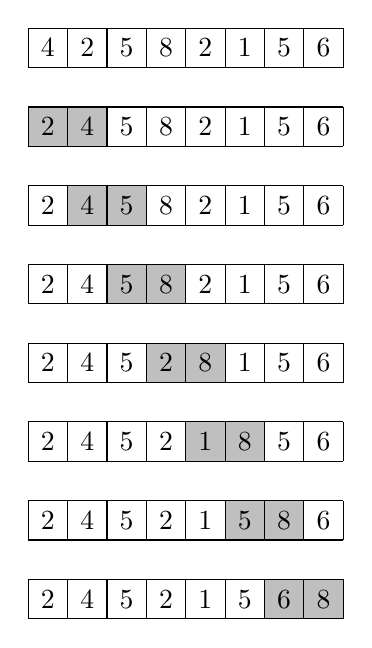
\begin{tikzpicture}[scale=0.5]
\begin{scope}
\draw (0,0) grid (8,1);
\foreach \x/\v in {0/4,1/2,2/5,3/8,4/2,5/1,6/5,7/6} \node at (0.5+\x,0.5) {\v};
\end{scope}
\begin{scope}[yshift=-2cm]
\fill[lightgray] (0,0) rectangle (2,1);
\draw (0,0) grid (8,1);
\foreach \x/\v in {0/2,1/4,2/5,3/8,4/2,5/1,6/5,7/6} \node at (0.5+\x,0.5) {\v};
\end{scope}
\begin{scope}[yshift=-4cm]
\fill[lightgray] (1,0) rectangle (3,1);
\draw (0,0) grid (8,1);
\foreach \x/\v in {0/2,1/4,2/5,3/8,4/2,5/1,6/5,7/6} \node at (0.5+\x,0.5) {\v};
\end{scope}
\begin{scope}[yshift=-6cm]
\fill[lightgray] (2,0) rectangle (4,1);
\draw (0,0) grid (8,1);
\foreach \x/\v in {0/2,1/4,2/5,3/8,4/2,5/1,6/5,7/6} \node at (0.5+\x,0.5) {\v};
\end{scope}
\begin{scope}[yshift=-8cm]
\fill[lightgray] (3,0) rectangle (5,1);
\draw (0,0) grid (8,1);
\foreach \x/\v in {0/2,1/4,2/5,3/2,4/8,5/1,6/5,7/6} \node at (0.5+\x,0.5) {\v};
\end{scope}
\begin{scope}[yshift=-10cm]
\fill[lightgray] (4,0) rectangle (6,1);
\draw (0,0) grid (8,1);
\foreach \x/\v in {0/2,1/4,2/5,3/2,4/1,5/8,6/5,7/6} \node at (0.5+\x,0.5) {\v};
\end{scope}
\begin{scope}[yshift=-12cm]
\fill[lightgray] (5,0) rectangle (7,1);
\draw (0,0) grid (8,1);
\foreach \x/\v in {0/2,1/4,2/5,3/2,4/1,5/5,6/8,7/6} \node at (0.5+\x,0.5) {\v};
\end{scope}
\begin{scope}[yshift=-14cm]
\fill[lightgray] (6,0) rectangle (8,1);
\draw (0,0) grid (8,1);
\foreach \x/\v in {0/2,1/4,2/5,3/2,4/1,5/5,6/6,7/8} \node at (0.5+\x,0.5) {\v};
\end{scope}
\end{tikzpicture}
\caption{Kuplajärjestämisen ensimmäinen kierros.}
\label{fig:kupjar}
\end{figure}

Kuva \ref{fig:kupjar} näyttää esimerkin kuplajärjestämisen ensimmäisestä
kierroksesta.
Kuplajärjestämisen ominaisuutena on, että $k$ kierroksen
jälkeen taulukon $k$ suurinta alkiota ovat oikeilla paikoillaan
taulukon lopussa.
Niinpä $n$ kierroksen jälkeen koko taulukko on järjestyksessä.

Voimme toteuttaa kuplajärjestämisen seuraavalla koodilla:

\begin{code}
for (int i = 0; i < n; i++) {
    for (int j = 0; j < n-1; j++) {
        if (taulu[j] > taulu[j+1]) {
            int x = taulu[j];
            taulu[j] = taulu[j+1];
            taulu[j+1] = x;
        }
    }
}
\end{code}

Kuplajärjestäminen muodostuu $n$ kierroksesta,
joista jokainen käy läpi taulukon,
joten algoritmi vie aikaa $O(n^2)$.

\subsection{Lisäysjärjestäminen}

\emph{Lisäysjärjestäminen} käy läpi taulukon vasemmalta oikealle
ja siirtää jokaisessa kohdassa olevaa alkiota vasemmalle
niin kauan kuin alkio on pienempi kuin sen vasemmalla
puolella oleva alkio.
Algoritmia voi myös ajatella niin,
että se varmistaa jokaisessa vaiheessa,
että taulukon $k$ ensimmäistä alkiota ovat oikeassa järjestyksessä.

\begin{figure}
\center
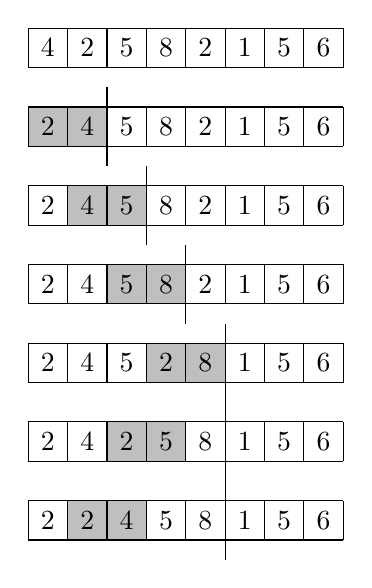
\begin{tikzpicture}[scale=0.5]
\begin{scope}
\draw (0,0) grid (8,1);
\foreach \x/\v in {0/4,1/2,2/5,3/8,4/2,5/1,6/5,7/6} \node at (0.5+\x,0.5) {\v};
\end{scope}
\begin{scope}[yshift=-2cm]
\fill[lightgray] (0,0) rectangle (2,1);
\draw (0,0) grid (8,1);
\foreach \x/\v in {0/2,1/4,2/5,3/8,4/2,5/1,6/5,7/6} \node at (0.5+\x,0.5) {\v};
\draw (2,-0.5) -- (2,1.5);
\end{scope}
\begin{scope}[yshift=-4cm]
\fill[lightgray] (1,0) rectangle (3,1);
\draw (0,0) grid (8,1);
\foreach \x/\v in {0/2,1/4,2/5,3/8,4/2,5/1,6/5,7/6} \node at (0.5+\x,0.5) {\v};
\draw (3,-0.5) -- (3,1.5);
\end{scope}
\begin{scope}[yshift=-6cm]
\fill[lightgray] (2,0) rectangle (4,1);
\draw (0,0) grid (8,1);
\foreach \x/\v in {0/2,1/4,2/5,3/8,4/2,5/1,6/5,7/6} \node at (0.5+\x,0.5) {\v};
\draw (4,-0.5) -- (4,1.5);
\end{scope}
\begin{scope}[yshift=-8cm]
\fill[lightgray] (3,0) rectangle (5,1);
\draw (0,0) grid (8,1);
\foreach \x/\v in {0/2,1/4,2/5,3/2,4/8,5/1,6/5,7/6} \node at (0.5+\x,0.5) {\v};
\draw (5,-0.5) -- (5,1.5);
\end{scope}
\begin{scope}[yshift=-10cm]
\fill[lightgray] (2,0) rectangle (4,1);
\draw (0,0) grid (8,1);
\foreach \x/\v in {0/2,1/4,2/2,3/5,4/8,5/1,6/5,7/6} \node at (0.5+\x,0.5) {\v};
\draw (5,-0.5) -- (5,1.5);
\end{scope}
\begin{scope}[yshift=-12cm]
\fill[lightgray] (1,0) rectangle (3,1);
\draw (0,0) grid (8,1);
\foreach \x/\v in {0/2,1/2,2/4,3/5,4/8,5/1,6/5,7/6} \node at (0.5+\x,0.5) {\v};
\draw (5,-0.5) -- (5,1.5);
\end{scope}
\end{tikzpicture}
\caption{Lisäysjärjestämisen ensimmäiset vaiheet.}
\label{fig:lisjar}
\end{figure}

Kuva \ref{fig:lisjar} näyttää esimerkin,
kuinka lisäysjärjestäminen aloittaa taulukon järjestämisen.
Jokaisessa kohdassa pystyviiva ilmaisee kohdan,
johon päättyy taulukon järjestyksessä oleva alkuosa.
Toisin kuin kuplajärjestämisessä, vierekkäisten alkioiden
vaihtamiset etenevät oikealta vasemmalle.

Seuraava koodi toteuttaa lisäysjärjestämisen:

\begin{code}
for (int i = 1; i < n; i++) {
    for (int j = i-1; j >= 0; j--) {
        if (taulu[j] > taulu[j+1]) {
            int x = taulu[j];
            taulu[j] = taulu[j+1];
            taulu[j+1] = x;
        } else break;
    }
}
\end{code}

Algoritmi muodostuu kahdesta sisäkkäisestä silmukasta,
joten sen aikavaativuus on $O(n^2)$.

\subsection{Inversiot}

Kuplajärjestäminen ja lisäysjärjestäminen ovat esimerkkejä
järjestämis\-algoritmeista, jotka perustuvat vierekkäisten
alkioiden vaihtamiseen.
Osoitamme seuraavaksi, että tällainen algoritmi ei voi \emph{koskaan}
toimia tehokkaammin kuin ajassa $O(n^2)$.

Hyödyllinen käsite järjestämisalgoritmien analysoinnissa
on \emph{inversio}: kaksi taulukossa olevaa alkiota,
jotka ovat väärässä järjestyksessä.
Tässä otetaan huomioon kaikki taulukon alkioparit,
ei vain vierekkäin olevia alkioita.
Esimerkiksi taulukossa $[3,1,4,2]$ on kolme inversiota:
$(3,1)$, $(3,2)$ ja $(4,2)$.

Taulukon inversioiden määrä kertoo, miten paljon työtä
vaaditaan sen järjestämiseen. Jos inversioiden määrä on 0,
taulukko on järjestyksessä.
Jos taas taulukko on käänteisessä järjestyksessä
suurimmasta pienimpään, sen inversioiden määrä on
\[
1 + 2 + \dots + (n-1) = \frac{n(n-1)}{2} = O(n^2).
\]

Aina kun vaihdamme taulukossa kahden vierekkäin olevan
alkion järjes\-tyksen, saamme poistettua taulukosta enintään
yhden inversion.
Niinpä jos taulukossa on $O(n^2)$ inversiota,
mikä tahansa vierekkäisiä alkioita vaihtava algoritmi
käyttää sen järjestämiseen aikaa ainakin $O(n^2)$.
Emme siis koskaan pysty luomaan tehokasta järjestämisalgoritmia,
jos rajoitumme vain vierekkäisten alkioiden vaihtamiseen keskenään.

\subsection{Vaihtojärjestäminen}

\emph{Vaihtojärjestäminen} etsii ensin taulukon pienimmän alkion
ja vaihtaa sen ensimmäiseksi.
Sitten se etsii taulukon loppuosan pienimmän alkion ja
vaihtaa sen toiseksi, jne., kunnes taulukko on järjestyksessä.
Kuva \ref{fig:vaijar} näyttää esimerkin
vaihtojärjestämisen toiminnasta.

\begin{figure}
\center
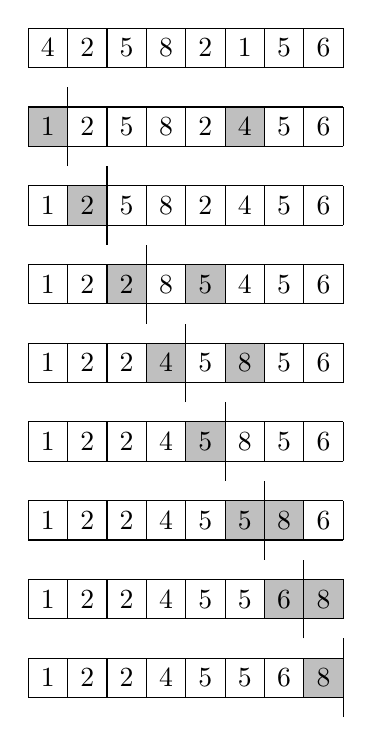
\begin{tikzpicture}[scale=0.5]
\begin{scope}
\draw (0,0) grid (8,1);
\foreach \x/\v in {0/4,1/2,2/5,3/8,4/2,5/1,6/5,7/6} \node at (0.5+\x,0.5) {\v};
\end{scope}
\begin{scope}[yshift=-2cm]
\fill[lightgray] (0,0) rectangle (1,1);
\fill[lightgray] (5,0) rectangle (6,1);
\draw (0,0) grid (8,1);
\foreach \x/\v in {0/1,1/2,2/5,3/8,4/2,5/4,6/5,7/6} \node at (0.5+\x,0.5) {\v};
\draw (1,-0.5) -- (1,1.5);
\end{scope}
\begin{scope}[yshift=-4cm]
\fill[lightgray] (1,0) rectangle (2,1);
\fill[lightgray] (1,0) rectangle (2,1);
\draw (0,0) grid (8,1);
\foreach \x/\v in {0/1,1/2,2/5,3/8,4/2,5/4,6/5,7/6} \node at (0.5+\x,0.5) {\v};
\draw (2,-0.5) -- (2,1.5);
\end{scope}
\begin{scope}[yshift=-6cm]
\fill[lightgray] (2,0) rectangle (3,1);
\fill[lightgray] (4,0) rectangle (5,1);
\draw (0,0) grid (8,1);
\foreach \x/\v in {0/1,1/2,2/2,3/8,4/5,5/4,6/5,7/6} \node at (0.5+\x,0.5) {\v};
\draw (3,-0.5) -- (3,1.5);
\end{scope}
\begin{scope}[yshift=-8cm]
\fill[lightgray] (3,0) rectangle (4,1);
\fill[lightgray] (5,0) rectangle (6,1);
\draw (0,0) grid (8,1);
\foreach \x/\v in {0/1,1/2,2/2,3/4,4/5,5/8,6/5,7/6} \node at (0.5+\x,0.5) {\v};
\draw (4,-0.5) -- (4,1.5);
\end{scope}
\begin{scope}[yshift=-10cm]
\fill[lightgray] (4,0) rectangle (5,1);
\fill[lightgray] (4,0) rectangle (5,1);
\draw (0,0) grid (8,1);
\foreach \x/\v in {0/1,1/2,2/2,3/4,4/5,5/8,6/5,7/6} \node at (0.5+\x,0.5) {\v};
\draw (5,-0.5) -- (5,1.5);
\end{scope}
\begin{scope}[yshift=-12cm]
\fill[lightgray] (5,0) rectangle (6,1);
\fill[lightgray] (6,0) rectangle (7,1);
\draw (0,0) grid (8,1);
\foreach \x/\v in {0/1,1/2,2/2,3/4,4/5,5/5,6/8,7/6} \node at (0.5+\x,0.5) {\v};
\draw (6,-0.5) -- (6,1.5);
\end{scope}
\begin{scope}[yshift=-14cm]
\fill[lightgray] (6,0) rectangle (7,1);
\fill[lightgray] (7,0) rectangle (8,1);
\draw (0,0) grid (8,1);
\foreach \x/\v in {0/1,1/2,2/2,3/4,4/5,5/5,6/6,7/8} \node at (0.5+\x,0.5) {\v};
\draw (7,-0.5) -- (7,1.5);
\end{scope}
\begin{scope}[yshift=-16cm]
\fill[lightgray] (7,0) rectangle (8,1);
\fill[lightgray] (7,0) rectangle (8,1);
\draw (0,0) grid (8,1);
\foreach \x/\v in {0/1,1/2,2/2,3/4,4/5,5/5,6/6,7/8} \node at (0.5+\x,0.5) {\v};
\draw (8,-0.5) -- (8,1.5);
\end{scope}
\end{tikzpicture}
\caption{Esimerkki vaihtojärjestämisen toiminnasta.}
\label{fig:vaijar}
\end{figure}

Seuraava koodi toteuttaa vaihtojärjestämisen:

\begin{code}
for (int i = 0; i < n; i++) {
    int k = i;
    for (int j = i; j < n; j++) {
        if (taulu[j] < taulu[k]) k = j;
    }
    int x = taulu[i];
    taulu[i] = taulu[k];
    taulu[k] = x;
}
\end{code}

Toisin kuin kuplajärjestäminen ja lisäysjärjestäminen,
vaihtojärjestäminen vaihtaa vain $O(n)$ alkiota keskenään
taulukossa, koska se siirtää aina pienimmän alkion
suoraan oikeaan kohtaan.
Algoritmi vie kuitenkin $O(n^2)$ aikaa,
koska jokaisen pienimmän alkion löytäminen vie $O(n)$ aikaa.

\section{Tehokkaat algoritmit}

Jos meillä on järjestettävänä suuri määrä tietoa,
$O(n^2)$-aikainen algoritmi ei kelpaa vaan tarvitsemme
tehokkaamman menetelmän.
Seuraavaksi tutustumme algoritmeihin,
joiden avulla voimme toteuttaa järjestämisen tehokkaasti $O(n \log n)$-ajassa.

\subsection{Lomitusjärjestäminen}

\emph{Lomitusjärjestäminen} on rekursiivinen järjestämisalgoritmi,
joka järjestää taulukon seuraavasti:

\begin{enumerate}
\item Jos taulukossa on vain yksi alkio,
älä tee mitään, koska taulukko on jo järjestyksessä.
\item Jaa taulukko keskeltä kahdeksi osataulukoksi ja järjestä
vasen ja oikea osataulukko rekursiivisesti.
\item Lomita vasen ja oikea osataulukko yhteen niin, että ne muodostavat
kokonaisen järjestetyn taulukon.
\end{enumerate}

Esimerkiksi jos järjestettävänä on taulukko $[4,2,5,8,2,1,5,6]$,
algoritmi jakaa sen ensin osataulukoiksi $[4,2,5,8]$ ja $[2,1,5,6]$.
Sitten algoritmi järjestää osataulukot rekursiivisesti,
jolloin tuloksena ovat taulukot $[2,4,5,8]$ ja $[1,2,5,6]$.
Lopuksi algoritmi lomittaa osataulukot takaisin yhteen
ja saa aikaan lopullisen järjestetyn taulukon $[1,2,2,4,5,5,6,8]$.

Lomitusjärjestämisen oleellisena osana on kahden järjestetyn osataulukon
lomittaminen. Tämä on mahdollista $O(n)$-ajassa, koska
voimme luoda uuden taulukon, johon alamme koota lopullista taulukkoa,
ja käydä järjestettyjä osataulukkoja läpi rinnakkain
vasemmalta oikealle ja valita aina pienimmän alkion seuraavaksi
lopulliseen taulukkoon.

\begin{figure}
\center
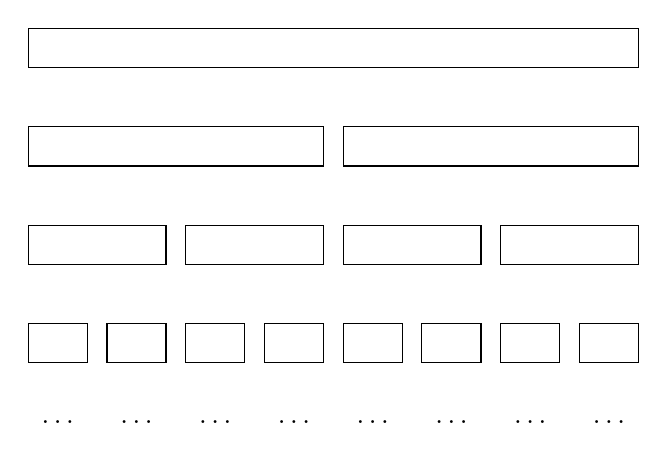
\begin{tikzpicture}[scale=0.5]
\draw (0+0.25,0) rectangle (16-0.25,1);
\foreach \x in {0,8} \draw (\x+0.25,-2.5) rectangle (\x+8-0.25,-1.5);
\foreach \x in {0,4,8,12} \draw (\x+0.25,-5) rectangle (\x+4-0.25,-4);
\foreach \x in {0,2,4,6,8,10,12,14} \draw (\x+0.25,-7.5) rectangle (\x+2-0.25,-6.5);
\foreach \x in {0,2,4,6,8,10,12,14} \node at (\x+1,-9) {$\dots$};
\end{tikzpicture}
\caption{Lomitusjärjestämisen toiminta esitettynä kerroksittain.}
\label{fig:lomjar}
\end{figure}

Kuinka tehokas lomitusjärjestäminen on?
Rekursiivisen algoritmin analysoinnissa auttaa esittää
algoritmin toiminta puuna,
jossa näkyvät tasoittain rekursiiviset kutsut.
Kuva \ref{fig:lomjar} näyttää tällaisen puun lomitusjärjestämisestä.
Koska taulukoiden koko puolittuu joka vaiheessa,
tasoja on yhteensä $O(\log n)$,
ja jokaisella tasolla lomittamiset vievät yhteensä aikaa $O(n)$.
Niinpä voimme todeta, että algoritmin aikavaativuus on $O(n \log n)$.

\subsection{Pikajärjestäminen}

Pikajärjestäminen on toinen rekursiivinen järjestämisalgoritmi,
joka toimii seuraavasti:

\begin{enumerate}
\item Jos taulukossa on vain yksi alkio,
älä tee mitään, koska taulukko on jo järjestyksessä.
\item Valitse jakoalkioksi jokin taulukossa oleva alkio $x$.
\item Siirrä jakoalkion vasemmalle puolelle kaikki $x$:ää pienemmät alkiot
ja oikealle puolelle kaikki $x$:ää suuremmat alkiot.
\item Järjestä jakoalkion eri puolilla olevat osataulukot rekursiivisesti.
\end{enumerate}

Pikajärjestäminen muistuttaa siis lomitusjärjestämistä,
mutta erona on, että taulukkoa ei jaeta kahdeksi yhtä suureksi
osataulukoksi vaan jaon määrää jakoalkio $x$.
Esimerkiksi jos haluamme järjestää taulukon $[4,2,5,8,2,1,5,6]$,
voimme valita jakoalkioksi vaikkapa taulukon ensimmäisen alkion $4$.
Kun siirrämme muut luvut jakoalkion eri puolille,
saamme osataulukot $[2,2,1]$ ja $[5,8,5,6]$, jotka järjestämme
sitten rekursiivisesti.

\begin{figure}
\center
\begin{tikzpicture}[scale=0.5]
\draw (0+0.25,0) rectangle (16-0.25,1);
\draw (0+0.25,-2.5) rectangle (1-0.25,-1.5);
\draw (1+0.25,-2.5) rectangle (16-0.25,-1.5);
\draw (1+0.25,-5) rectangle (2-0.25,-4);
\draw (2+0.25,-5) rectangle (16-0.25,-4);
\draw (2+0.25,-7.5) rectangle (3-0.25,-6.5);
\draw (3+0.25,-7.5) rectangle (16-0.25,-6.5);
\foreach \x in {4,8,12} \node at (\x+1,-9) {$\dots$};
\end{tikzpicture}
\caption{Pikajärjestämisen huonoin tapaus: jokaisessa vaiheessa lähes kaikki
alkiot jäävät toiseen osataulukkoon.}
\label{fig:pikjar}
\end{figure}

Jakoalkion valinnan jälkeen pystymme siirtämään lineaarisessa ajassa
alkiot jakoalkion eri puolille.
Pikajärjestämisen tehokkuuden ratkaisee, kuinka tasaisesti
alkiot jakautuvat osataulukoiksi.
Parhaassa tapauksessa joka vaiheessa saamme kaksi suunnilleen
yhtä suurta osataulukkoa, jolloin tilanne vastaa kuvaa \ref{fig:lomjar}.
Kuitenkin on myös mahdollista, että jaot ovat epätasaisia ja
joka vaiheessa lähes kaikki alkiot jäävät toiselle puolelle.
Kuva \ref{fig:pikjar} näyttää esimerkin tällaisesta tilanteesta.

Parhaassa tapauksessa pikajärjestäminen toimii siis yhtä nopeasti
kuin lomitusjärjestäminen eli ajassa $O(n \log n)$.
Pahimmassa tapauksessa aikaa kuluu kuitenkin $O(n^2)$,
koska algoritmin suorituksessa saattaa muodostua $O(n)$ tasoa,
joista jokainen vie aikaa $O(n)$.
Miksi haluaisimme siis käyttää pikajärjestämistä,
joka toimii \emph{ehkä} ajassa $O(n \log n)$,
kun voisimme käyttää sen sijasta lomitusjärjestämistä,
joka toimii \emph{varmasti} ajassa $O(n \log n)$?

Ensinnäkin pikajärjestäminen toimii \emph{yleensä}
ajassa $O(n \log n)$, kunhan valitsemme jakoalkion huolellisesti.
Taulukon ensimmäinen alkio ei ole käytän\-nössä hyvä jakoalkio,
koska silloin esimerkiksi valmiiksi järjestyksessä olevan
taulukon käsittely vie aikaa $O(n^2)$.
Parempi tapa on esimerkiksi ottaa tarkasteluun taulukon ensimmäinen,
keskimmäinen ja viimeinen alkio ja valita niistä
järjestyksessä keskimmäinen jakoalkioksi.
Tällaisella jakoalkion valinnalla on jo vaikeaa keksiä taulukkoa,
jossa pikajärjestäminen veisi aikaa $O(n^2)$,
saati sitten että tällainen tilanne esiintyisi käytännössä.

Pikajärjestämisen todellinen etu on kuitenkin siinä,
että sen vakiokertoimet ovat pienet.
Vaikka lomitusjärjestäminen ja pikajärjestäminen vievät molemmat
aikaa $O(n \log n)$, kokemus on osoittanut, että
pikajärjestäminen toimii yleensä käytännössä nopeammin.
Yksi syy tähän on, että pikajärjestä\-minen siirtää vähemmän
alkioita ympäri taulukkoa: aina kun alkiot on siirretty
jakoalkion eri puolille, niitä ei siirretä enää koskaan
jakoalkion yli.

\subsection{Järjestämisen alaraja}

Onko mahdollista luoda järjestämisalgoritmi, joka toimisi
nopeammin kuin $O(n \log n)$?
Tämä ei ole mahdollista, jos oletamme, että algoritmin
tulee perustua taulukon alkioiden vertailuihin.

Voimme ajatella vertailuihin perustuvaa järjestämistä
prosessina, jossa jokainen vertailu antaa meille tietoa
taulukosta ja saamme vietyä taulukkoa lähemmäs järjestystä.
Oletamme seuraavaksi, että taulukko muodostuu luvuista
$1,2,\dots,n$, jolloin meillä on $n!$ vaihtoehtoa, mikä
on taulukon alkuperäinen järjestys.
Jotta järjestämisalgoritmi voisi toimia oikein,
sen täytyy käsitellä jokainen järjestys eri tavalla.

Esimerkiksi jos $n=3$, taulukon mahdolliset järjestykset alussa ovat
$[1,2,3]$, $[1,3,2]$, $[2,1,3]$, $[2,3,1]$, $[3,1,2]$ ja $[3,2,1]$.
Algoritmi voi vertailla ensin vaikkapa ensimmäistä ja toista alkiota.
Jos ensimmäinen alkio on pienempi, voimme päätellä,
että mahdolliset taulukot ovat $[1,2,3]$, $[1,3,2]$ ja $[2,3,1]$.
Jos taas ensimmäinen alkio on suurempi,
mahdolliset taulukot ovat $[2,1,3]$, $[3,1,2]$ ja $[3,2,1]$.
Tämän jälkeen voimme jatkaa vertailuja ja saada lisää tietoa taulukosta.
Algoritmi voi päättyä vasta silloin, kun jäljellä on vain yksi
mahdollinen taulukko, jotta voimme olla varmoja, että olemme
järjestäneet taulukon oikein.

Tärkeä seikka on, että jokaisessa vertailussa ainakin toisessa
tapauksessa meille jää jäljelle puolet mahdollisista taulukoista.
Niinpä jos algoritmilla käy huono tuuri, se voi enintään puolittaa
taulukoiden määrän joka askeleella.
Tämä tarkoittaa, että pahimmassa tapauksessa algoritmi joutuu
tekemään luokkaa $\log_2(n!)$ vertailua.
Logaritmien laskusääntöjen perusteella
\[
\log_2(n!) = \log_2(1)+\log_2(2)+\dots+\log_2(n).
\]
Saamme tälle summalle alarajan ottamalla huomioon vain
$n/2$ viimeistä termiä ja arvioimalla niitä alaspäin niin, 
että jokaisen termin suuruus on vain $\log_2(n/2)$. Tuloksena on alaraja
\[
\log_2(n!) \ge (n/2) \log_2(n/2),
\]
mikä tarkoittaa, että algoritmi joutuu
tekemään $\Omega(n \log n)$ vertailua pahimmassa tapauksessa.

\subsection{Laskemisjärjestäminen}

Laskemisjärjestäminen on $O(n)$-aikainen järjestämisalgoritmi,
jonka toiminta perustuu oletukseen, että taulukon alkiot
ovat sopivan pieniä kokonaislukuja.
Tarkemmin ottaen algoritmi olettaa, että jokainen luku on
kokonaisluku välillä $0 \dots k$, missä $k=O(n)$.

Algoritmissa on ideana luoda \emph{kirjanpito}, joka kertoo,
montako kertaa mikäkin mahdollinen luku välillä $0 \dots k$
esiintyy taulukossa.
Tällaista kirjanpitoa varten voimme määritellä taulukon
\texttt{kerrat}, jossa $\texttt{kerrat}[x]$ ilmaisee,
montako kertaa luku $x$ esiintyy taulukossa.
Saamme luotua kirjanpidon käymällä läpi taulukon sisällön,
ja sitten voimme muodostaa järjestetyn taulukon
kirjanpidon perusteella.
Seuraava koodi havainnollistaa asiaa:

\begin{code}
for (int i = 0; i < n; i++) {
    kerrat[taulu[i]]++;
}
int i = 0;
for (int x = 0; x <= k; x++) {
    for (int j = 0; j < kerrat[x]; j++) {
        taulu[i] = x;
        i++;
    }
}
\end{code}

Algoritmin molemmat vaiheet vievät aikaa $O(n)$,
joten se toimii ajassa $O(n)$.
Algoritmi on kuitenkin käyttökelpoinen vain silloin,
kun raja $k$ on niin pieni, että voimme pitää
muistissa kirjanpitoa.

\section{Järjestäminen Javassa}

Vaikka on hyödyllistä tuntea järjestämisen teoriaa,
käytännössä ei ole hyvä idea toteuttaa itse
järjestämisalgoritmia, koska nykypäivän ohjelmointikielissä
on valmiit työkalut järjestämiseen.
Esimerkiksi Javassa voimme käyttää metodia \texttt{Arrays.sort},
joka järjestää sille annetun taulukon:

\begin{code}
int[] taulu = {4,2,5,8,2,1,5,6};
Arrays.sort(taulu);
\end{code}

Kiinnostava kysymys on, mitä algoritmia Java käyttää
taulukon järjes\-tämiseen.
Yllättävää kyllä, tämä riippuu siitä, minkä tyyppistä tietoa
taulukossa on.
Jos taulukon alkiot ovat alkeistyyppisiä
(esimerkiksi \texttt{int}), Java käyttää 
pikajärjestämisen muunnelmaa.
Jos taas alkiot ovat oliotyyppisiä
(esimerkiksi \texttt{String}),
algoritmina on lomitusjärjestäminen.

Jos haluamme, että Java pystyy järjestämään omia olioitamme,
meidän täytyy toteuttaa luokkaan metodi \texttt{compareTo} ja
merkitä, että luokka toteuttaa rajapinnan \texttt{Comparable}.
Kun \texttt{Arrays.sort} järjestää taulukon,
se kutsuu metodia \texttt{compareTo} aina, kun se haluaa selvittää
kahden alkion suuruusjärjestyksen.
Metodin tulee palauttaa negatiivinen arvo, nolla tai positiivinen arvo
sen mukaan, onko olio itse pienempi, yhtä suuri vai suurempi
kuin parametrina annettu olio.

Esimerkiksi seuraava koodi toteuttaa luokan \texttt{Piste},
johon voidaan tallentaa pisteen x- ja y-koordinaatit.
Luokassa on metodi \texttt{compareTo}, joka määrittelee,
että pisteet järjestetään ensisijaisesti x-koordinaatin ja
toissijaisesti y-koordinaatin mukaan.

\begin{code}
public class Piste implements Comparable<Piste> {
    public int x, y;

    public int compareTo(Piste p) {
        if (this.x != p.x) return this.x-p.x;
        else return this.y-p.y;
    }
}
\end{code}

Metodin \texttt{compareTo} avulla voimme myös konkreettisesti
tarkastella, mitä Java tekee järjestäessään taulukon.
Seuraava luokka sisältää vain yhden luvun,
mutta ilmoittaa meille aina, kun Java kutsuu
\texttt{compareTo}-funktiota:

\begin{code}
public class Luku implements Comparable<Luku> {
    public int luku;

    public int compareTo(Luku x) {
        System.out.println("vertailu: " + luku + " " + x.luku);
        return this.luku-x.luku;
    }
}
\end{code}

Esimerkiksi kun järjestettävänä taulukkona on $[4,1,3,2]$,
saamme tietää, että Java tekee seuraavat vertailut:

\begin{code}
vertailu: 1 4
vertailu: 3 1
vertailu: 3 4
vertailu: 3 1
vertailu: 2 3
vertailu: 2 1
\end{code}

\section{Esimerkki: Keskiluvut}

Annettuna on $n$ kokonaisluvun taulukko ja haluamme
laskea sille mediaanin ja moodin.
\emph{Mediaani} on keskimmäinen arvo, kun taulukko järjestetään
pienimmästä suurimpaan.
\emph{Moodi} taas on arvo, joka esiintyy useimmiten taulukossa.
Esimerkiksi taulukon $[2,1,3,1,5]$ mediaani on 2 ja moodi on 1.

Pystymme laskemaan sekä mediaanin että moodin tehokkaasti
$O(n \log n)$-ajassa järjestämisen avulla.
Mediaanin laskeminen on erityisen helppoa,
koska meidän riittää järjestää taulukko ja valita
sieltä keskimmäinen luku. Seuraava metodi hoitaa asian:

\begin{code}
int mediaani(int[] taulu) {
    Arrays.sort(taulu);
    return taulu[taulu.length/2];
}
\end{code}

Tässä tulkintana on, että kun $n$ on parillinen, mediaani
on kahdesta keskimmäisestä luvusta pienempi.

Moodin laskemisessa auttaa havainto, että taulukon järjestämisen
jälkeen kaikki yhtä suuret luvut ovat vierekkäin.
Niinpä voimme ensin järjestää taulukon ja etsiä sitten siitä
pisimmän samaa lukua toistavan osuuden.
Seuraava metodi toimii näin:

\begin{code}
int moodi(int[] taulu) {
    Arrays.sort(taulu);
    int tulos = taulu[0];
    int pituus = 1;
    int paras = 1;
    for (int i = 1; i < taulu.length; i++) {
        if (taulu[i-1] != taulu[i]) pituus = 0;
        pituus++;
        if (pituus > paras) {
            paras = pituus;
            tulos = taulu[i];
        }
    }
    return tulos;
}
\end{code}

Huomaa, että koska taulukko välitetään viittauksena metodeille,
taulukon uusi järjestys jää voimaan metodien kutsumisen jälkeen
eli metodeilla on \emph{sivuvaikutuksia}.
Seuraava koodi havainnollistaa asiaa:

\begin{code}
int[] taulu = {2,1,3};
System.out.println(mediaani(taulu)); // 2
System.out.println(taulu[0]); // 1
\end{code}

Koodi laskee taulukon mediaanin, jolloin taulukko
myös järjestyy. Niinpä taulukon kohdassa 0 oleva luku
on mediaanin laskemisen jälkeen 1.

Jos emme halua metodiin sivuvaikutuksia voimme metodin
alussa tehdä kopion taulukosta ja järjestää sen alkuperäisen
taulukon sijasta. Voimme tehdä kopion seuraavasti \texttt{clone}-metodilla:

\begin{code}
int[] kopio = taulu.clone();
Arrays.sort(kopio);
...
\end{code}

Tämän jälkeen mediaanin laskeminen ei
muuta taulukon sisältöä:

\begin{code}
int[] taulu = {2,1,3};
System.out.println(mediaani(taulu)); // 2
System.out.println(taulu[0]); // 2
\end{code}
